\documentclass[a4paper, 11pt]{article}
\usepackage[utf8]{inputenc} % Change according your file encoding
\usepackage{graphicx}
\usepackage{url}
\usepackage{booktabs}
\usepackage{float}
\graphicspath{{../}}


%opening
\title{Seminar Report: seminar Opty}
\author{Rodrigo Arias Mallo}
\date{2017U2}

\begin{document}

\maketitle

\section{Introduction}

This seminar consists of a set of experiments of a Erlang server implementing a 
optimistic concurrency control, with backward validation, to access a database. 

\section{Work done}

Some experiments have been designed to measure how different parameters affect 
the performance of the server.

Each experiment that shares the same source code is designed by a number. Each 
subexperiment where only the parameters are changed, belongs to the same 
experiment number, and is identified by a letter. This structure allows batch 
processing of all the experiments, and a change in the source code automatically 
produces an update on the subexperiments.

This hierarchy is controlled by Makefiles, which are programed to run all the 
experiments, produce the figures, and compile this document with the results in 
figures.

This design provides reproducible results. Some deviation may occur, as the seed 
was not fixed, and the concurrent process behavior is not predictable.

\newpage
\section{Experiments}

In all the experiments the average of the success rate is plotted by a line, and 
also the standard deviation in the success rate of each client. For each 
measurement, there are some comments about the explanation of the system based 
on the observed behavior.

\subsection{Experiment 1}

Some set of experiments are performed to measure the performance of the 
transaction server. Each experiment is designed by a name like 
\texttt{exp1$\alpha$} where $\alpha$ is a letter.

\begin{table}[H]
\centering
\begin{tabular}{c c c c c c}
\toprule
Exp.						&	Clients	&	Entries	&	Reads & Writes	& Time (s)	\\
\midrule
\texttt{exp1a}	&	$C$			&	10			& 10		&	10			&	3					\\
\texttt{exp1b}	&	10			&	$E$			& 10		&	10			&	3					\\
\texttt{exp1c}	&	10			&	10			& $R$		&	10			&	3					\\
\texttt{exp1d}	&	10			&	10			& 10		&	$W$			&	3					\\
\texttt{exp1e}	&	10			&	10			& 10		&	10			&	$T$				\\
\texttt{exp1f}	&	10			&	10			& $i$		&	$20-i$	&	3					\\
\bottomrule
\end{tabular}
\end{table}

With $C,E,R,W \in [1,20]$, $T \in [1,10]$ and $i \in [0,20]$.

\paragraph{\texttt{exp1a}: Clients vs Success rate.}

As more clients try to access the database more transactions conflicts appear, 
so the average success rate decreases as they grow. Also, the success rate for 
each client is similar between clients.

\begin{figure}[H]
\centering
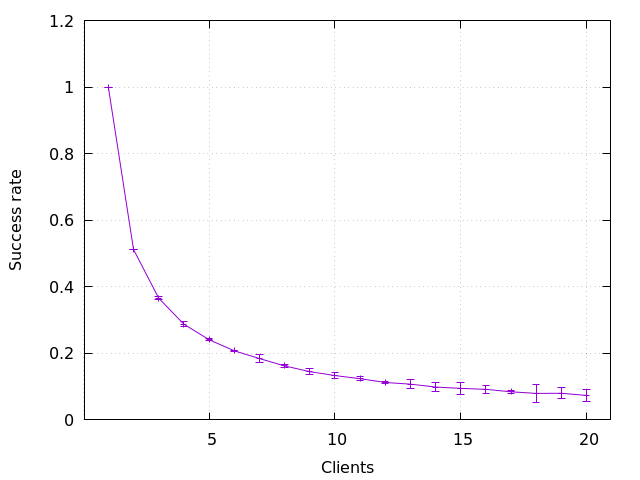
\includegraphics[width=.8\linewidth]{exp1/a/fig.png}
\end{figure}

\paragraph{\texttt{exp1b}: Entries vs Success rate}

The average success rate decreases as the entries grow, until they reach the 
value 10. Then, the success rate starts to grow slowly. We observe a increasing 
deviation in the success rate with 3 and 4 entries. The other runs show small 
deviations.
\nopagebreak
\begin{figure}[H]
\centering
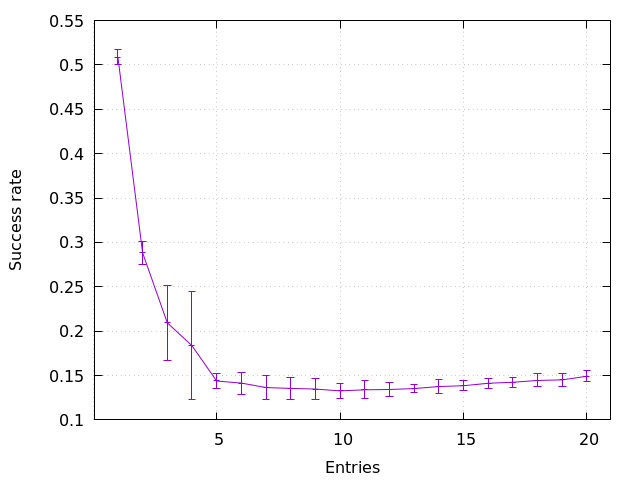
\includegraphics[width=.8\linewidth]{exp1/b/fig.png}
\end{figure}

\paragraph{\texttt{exp1c}: Reads vs Success rate}

As the number of reads performed by the clients increases, more transactions are 
in conflict, so the success rate is reduced. The deviation increases as the 
number of reads increases.
\nopagebreak
\begin{figure}[H]
\centering
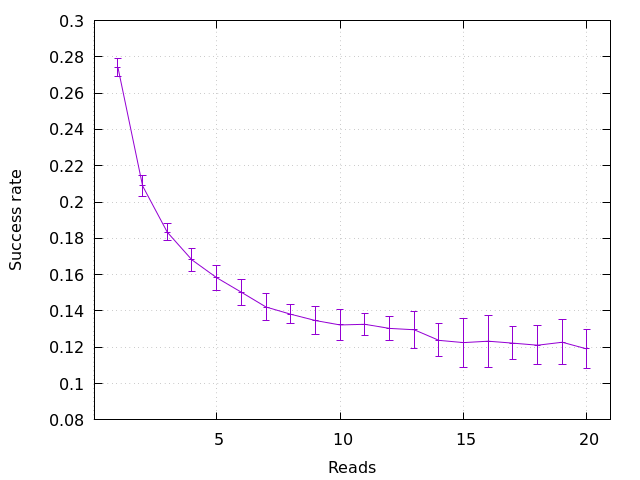
\includegraphics[width=.8\linewidth]{exp1/c/fig.png}
\end{figure}

\paragraph{\texttt{exp1d}: Writes vs Success rate}

As the number of writes performed by the clients increases, more transactions 
are in conflict, so the success rate is reduced. The deviation increases with 
the number of writes.
\nopagebreak
\begin{figure}[H]
\centering
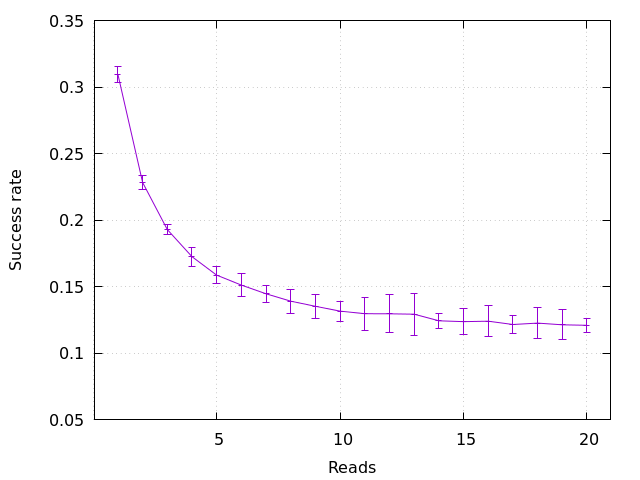
\includegraphics[width=.8\linewidth]{exp1/d/fig.png}
\end{figure}

\paragraph{\texttt{exp1e}: Time vs Success rate}

As the time allowed to the simulation grows, there seems that the success rate 
is not affected. The deviation seems to decrease as the time grows.
\nopagebreak
\begin{figure}[H]
\centering
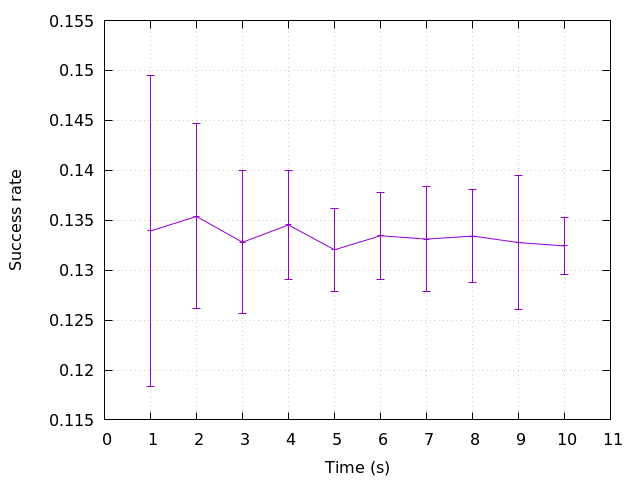
\includegraphics[width=.8\linewidth]{exp1/e/fig.png}
\end{figure}

\newpage
\paragraph{\texttt{exp1f}: Ratio R/W vs Success rate}

Let $R$ be the number of reads, then the number of writes is defined as $W = 20 
- R$.  When the number of reads or writes is 0, we have no conflicts.  But as 
the ratio is close to $1/2$ the performance is worse.  The deviation is small.
\nopagebreak
\begin{figure}[H]
\centering
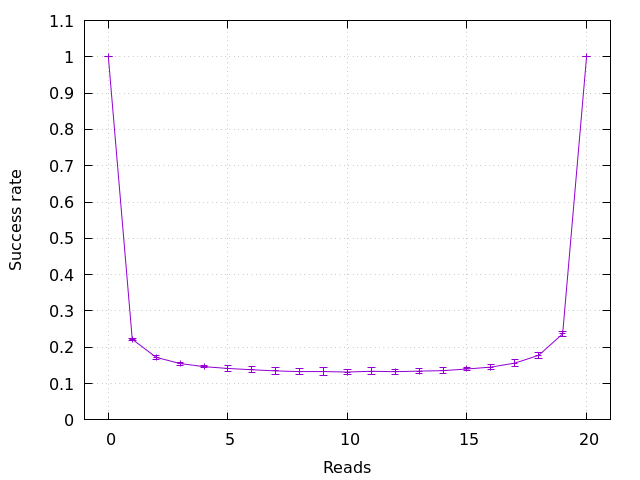
\includegraphics[width=.8\linewidth]{exp1/f/fig.png}
\end{figure}

\subsection{Experiment 2}

The experiment \texttt{exp2a} modifies the behavior of the client in order to 
access only a random subset of the entries of the database. Each client 
maintains a subset of size $A$, which is randomly selected from all the entries.
The size of the subset $A$ is tested with values in $[1, 20]$ for a database of 
20 elements.

\newpage
\paragraph{\texttt{exp2a}: Access subset size vs Success rate}

There can be shown that the performance decreases as the access subset grows.  
The deviation between clients is small.

\nopagebreak
\begin{figure}[H]
\centering
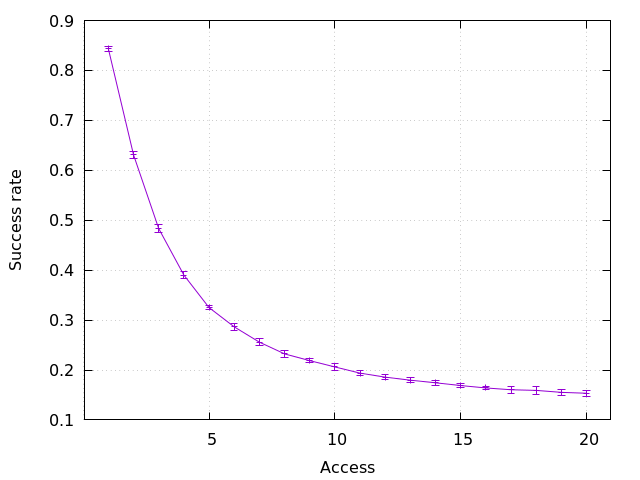
\includegraphics[width=.8\linewidth]{exp2/a/fig.png}
\end{figure}


%\section{Open questions}

%\textit{Try to answer all the open questions in the documentation. When 
%possible, do experiments to support your answers.}

\section{Personal opinion}

Erlang is a bottleneck. I have spent about 90\% of the time figuring out how to 
instruct the language to do what I wanted. Please look for a simpler 
alternative. Maybe Go is simple and stable enough. Or maybe you can provide a 
simple program with a graphical simulation to understand what happens.

\end{document}
